\newpage
\section{Aufbau und Durchführung}
\label{sec:Durchfuehrung}
\subsection{Aufbau des Germanium-Detektors}
Der Querschnitt des verwendeten Detektors ist in Abbildung \ref{fig:Detektor} zu sehen.
Er ist zylinderförmig aufgebaut und besitzt eine mit Lithium-Atomen n-dotierte Oberfläche und eine mit Gold-Atomen p-dotierte Innenfläche.
Der Detektor ist für eine gute thermische Isolierung von einer Aluminiumhaube gekapselt, weswegen erst ab einer bestimmten Energie $\gamma-$Quanten registriert werden können (Empfindlichkeitsgrenze).
 \begin{figure}
   \centering
   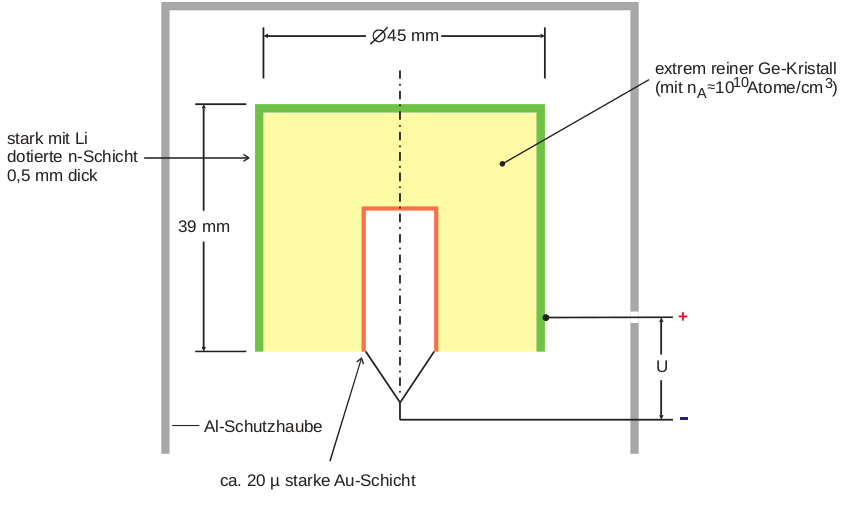
\includegraphics[height=9cm]{content/Detektor.png}
   \caption{Aufbau des Ge-Detektors.\cite{V18}}
   \label{fig:Detektor}
 \end{figure}
\subsection{Elektronische Schaltung}
Der Detektor nimmt Ladungsimpulse wahr, die proportional zur eingehenden Energie der $\gamma-$Quanten sind.
Ein rückgekoppelter Operationsverstärker erzeugt durch elektrische Integration einen proportionalen Spannungspegel.
Der dafür benutzte Integrationskondensator muss nach jedem Quantennachweis regelmäßig entladen werden, da die Spannung sonst stufenförmig steigen würde und eine Höhenanalyse nicht möglich wäre.
Das geschieht durch eine optoelektronische Rückkopplung.
All dies bildet den Vorverstärker, welcher im Aluminiumgehäuse sitzt.

Nach dem Vorverstärker ist der Hauptverstärker angeschlossen.
Der Hauptverstärker normiert die empfangenen Spannungssignale auf eine Höhe von $0$ bis $\SI{10}{\volt}$, damit der Analog-Digital-Converter (ADC) brauchbare Daten verarbeiten kann.
Als pile-up wird das aufsummieren von Impulsen bezeichnet, die in einem kurzen Zeitintervall registriert werden.
Damit der dadurch viel zu hohe Impuls das Energie-Spektrum nicht verfälscht sperrt der Hauptverstärker für eine kurze Zeit den ADC.
Infolge dessen wird eine kleine Zählrate nicht registriert, weswegen eine eventuelle Totzeit-Korrektur für die Auswertung notwendig ist.

Das Signal gelangt vom Hauptverstärker schließlich in den Vielkanal-Analysator, der die Impulse nach ihrer Höhe und Häufigkeit sortiert.
Die Daten werden auf verschiedenen Kanälen gespeichert und ein angeschlossener Computer zeigt die gemessenen Signale als Impulshöhenspektrum dar.
Das beschriebene Schaltbild ist in Abbildung \ref{fig:Schaltung} zu sehen.
 \begin{figure}
   \centering
   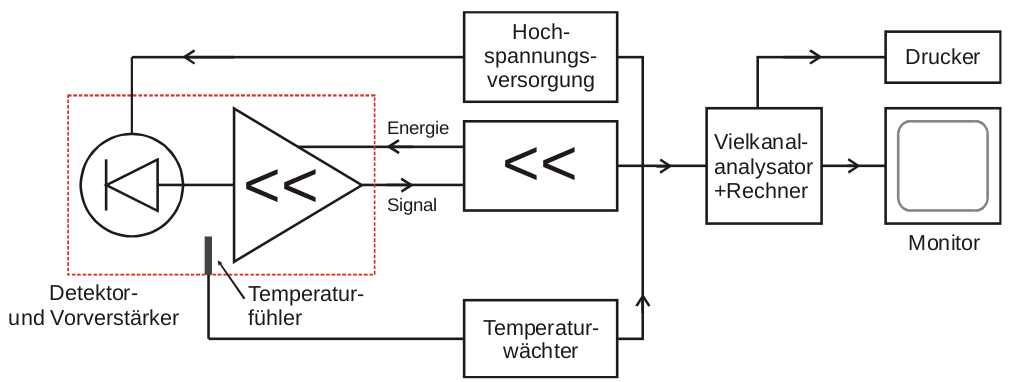
\includegraphics[height=5.5cm]{content/Schaltung.png}
   \caption{Schaltung der verwendeten Messapparatur.\cite{V18}}
   \label{fig:Schaltung}
 \end{figure}
\subsection{Energie- und Aktivitätsbestimmung}
Um die im Experiment gemessenen Daten auswerten zu können ist zunächst eine Kalibrierung des Detektors erforderlich.
Dazu ist es nötig das Spektrum eines bereits bekannten $\gamma-$Strahlers zu betrachten.
Hier ist der Zusammenhang von Spektrallinien und den zugehörigen Energien schon gegeben.
Durch eine lineare Ausgleichsrechnung kann eine Zuordnung der Kanalnummer zu den Energiewerten geschehen.

Die Nachweiswahrscheinlichkeit des Detektors errechnet sich aus der Formel
\begin{equation}
\label{eqn:eff} 
Q = 4\pi\,\cdot Z\,(\Omega\cdot A\cdot W\cdot t_{\symup{mess}})^{-1}.
\end{equation}
Hier steht W für die Emissionswahrscheinlichkeit einer bestimmten $\gamma-$Energie, $Z$ für die Summe der Impulse, $A$ für die Aktivität des Strahlers, $\Omega$ für den Raumwinkel, unter dem der Detektor den Strahler sieht und $t_{\symup{mess}}$ für die Messzeit.

Die Aktivität des Strahlers ist vom Hersteller angegeben und wird für unbekannte Nuklide später selber bestimmt.
Der Raumwinkel $\Omega$ errechnet sich aus
\begin{equation}
\label{eqn:raum}
\frac{\Omega}{4\pi}=\frac12\left(1-\frac a{\sqrt{a²+r²}}\right).
\end{equation}
Der Radius des Detektors $r$ ist in Abbildung \ref{fig:Detektor} einzusehen und $a$ ist der Abstand zwischen Detektor und Strahler.
\subsection{Durchführung}
Um die Kalibrierung des Detektors vornehmen zu können wird zunächst das bekannte Spektrum eines $\ce{^{152}}\symup{Eu}$-Strahlers aufgenommen.
Daraufhin wird das Spektrum des $\ce{^{137}}\symup{Cs}$-Strahlers gemessen.
Darin wird versucht das Compton-Kontinuum, den Rückstreupeak und den Photopeak zu erkennen.
Bei dem dritten untersuchten Strahler soll bestimmt werden ob es sich um $\ce{^{125}}\symup{Sb}$ oder $\ce{^{133}}\symup{Ba}$ handelt.
Abschließend wird ein unbekannter Strahler untersucht aus dessen Spektrum eine Nuklidbestimmung erfolgt.
Jeder Strahler wird ungefähr eine Stunde lang gemessen.